\documentclass{article}
\pagestyle{empty}
\usepackage{tikz}
\usetikzlibrary{arrows.meta,decorations.pathreplacing}
\definecolor{diagOrange}{RGB}{240,105,26}
\definecolor{boxFill}{RGB}{239,239,239}
\definecolor{boxStroke}{RGB}{154,154,154}
\definecolor{inkGray}{RGB}{51,51,51}
\begin{document}
\noindent
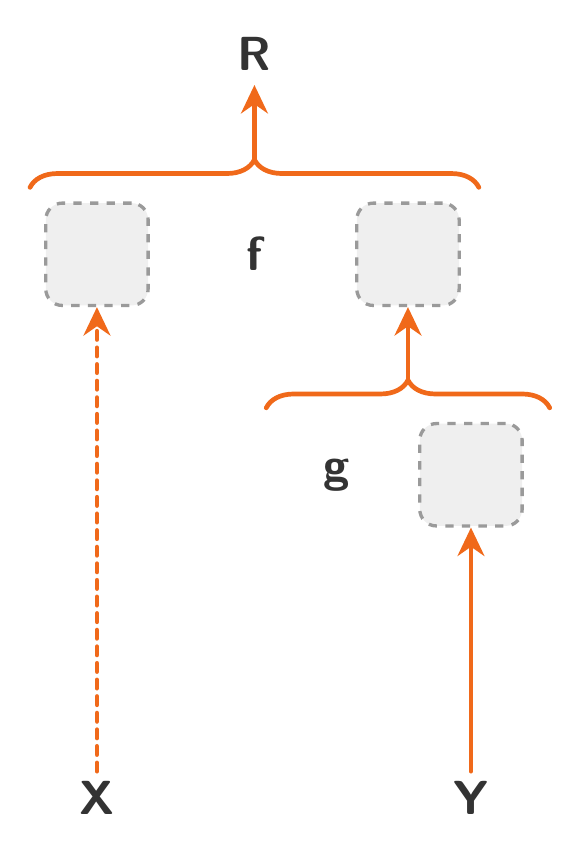
\begin{tikzpicture}[
  >={Stealth[length=3.6mm,width=3.4mm]},
  line join=round,
  slot/.style={draw=boxStroke, dashed, line width=1.2pt, rounded corners=6pt,
               fill=boxFill, minimum size=1.3cm},
  flow/.style={diagOrange, line width=1.7pt, line cap=round, ->},
  flowdash/.style={diagOrange, line width=1.7pt, line cap=round, dashed, ->},
  brace/.style={diagOrange, line width=1.7pt, line cap=round,
                decorate, decoration={brace, amplitude=10pt}},
  lbl/.style={inkGray, font=\sffamily\bfseries\LARGE},
]
  % inputs (same bottom level)
  \node[lbl] (X) at (2.15,-1.5) {X};
  \node[lbl] (Y) at (6.9,-1.5) {Y};

  % f's two argument slots + brace (label centred)
  \node[slot] (fLs) at (2.15,5.4) {};
  \node[slot] (fRs) at (6.1,5.4) {};
  \draw[brace] (1.3,6.25) -- (7.0,6.25);   % tip at x=4.15
  \node[lbl] at (4.15,5.4) {f};

  % g's argument slot + brace (label left, slot right)
  \node[slot] (gSlot) at (6.9,2.6) {};
  \draw[brace] (4.3,3.45) -- (7.9,3.45);   % tip at x=6.1
  \node[lbl] at (5.2,2.6) {g};

  % wiring (add "mirror" to a brace decoration if its tip points down)
  \draw[flowdash] (X) -- (fLs);            % X -> f's left slot (long dashed riser)
  \draw[flow]     (Y) -- (gSlot);          % Y -> g
  \draw[flow] (6.1,3.78) -- (fRs);         % g -> f's right slot
  \draw[flow] (4.15,6.58) -- (4.15,7.55);  % f -> R
  \node[lbl] (R) at (4.15,7.95) {R};
\end{tikzpicture}
\end{document}
